\subsection{Reflection, Transmission and Absorbance}

\begin{frame}{Reflection, Transmission, Absorbance}
    \begin{columns}
        \column{0.55\textwidth}
        \vspace{-2mm}
        Snell's law: \( ( n \approx \sqrt{\varepsilon} )\)
        \begin{equation*}
            \theta_I = \theta_R, \ \ n_1 \sin \theta_I = n_2 \sin \theta_T.
        \end{equation*}
        
        TE mode: (\(\mathbf{E} \perp \text{Plane of incidence} \)) 
        \begin{equation*}
                R = \left[ \dfrac{ n_1 \cos \theta_I - \sqrt{ n_2^2 - n_1^2 \sin^2 \theta_I} }{ n_1 \cos \theta_I + \sqrt{n_2^2 - n_1^2 \sin^2 \theta_I}} \right]^2.
        \end{equation*}

        TM mode: (\(\mathbf{E} \parallel \text{Plane of incidence} \)) 
        \begin{equation*}
                R = \left[ \dfrac{ n_2 \cos \theta_I - \sqrt{ n_2^2 - n_1^2 \sin^2 \theta_I} }{ n_2 \cos \theta_I + \sqrt{n_2^2 - n_1^2 \sin^2 \theta_I}} \right]^2.
        \end{equation*}

        \column{0.45\textwidth}
        \vspace{-8mm}
        \begin{figure}
            \centering
            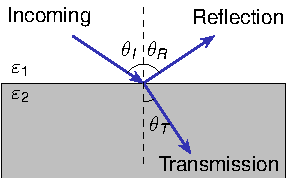
\includegraphics[width=\textwidth]{Figures/Reflection_Transmission.pdf}
            \caption{Reflection, Transmission.}
            \label{fig:Reflection_Transmission}
        \end{figure}
        \vspace{-2mm}
        \begin{figure}
            \centering
            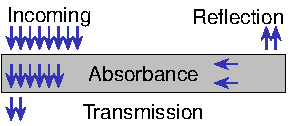
\includegraphics[width=\textwidth]{Figures/Absorbance.pdf}
            \caption{Absorbance.}
            \label{fig:Absorbance}
        \end{figure}
    \end{columns}
\end{frame}